%!TEX root = ../mfilters.tex
\subsection{Задание 4. Зависимость отношения сигнал/шум на выходе согласованного
фильтра от параметров входного сигнала}

В задании исследуется свойство системы с согласованным фильтром при различных
параметрах ЛЧМ сигнала: девиации частоты $\Delta f_{\text{дев}}$ и длительности
сигнала $\tau$.




\subsubsection{Изменяющаяся длительность ЛЧМ сигнала}%
\label{ssub:izmeniaiushchaiasia_dlitel_nost_signala_tau_}

\begin{figure}[h!]
    \centering
    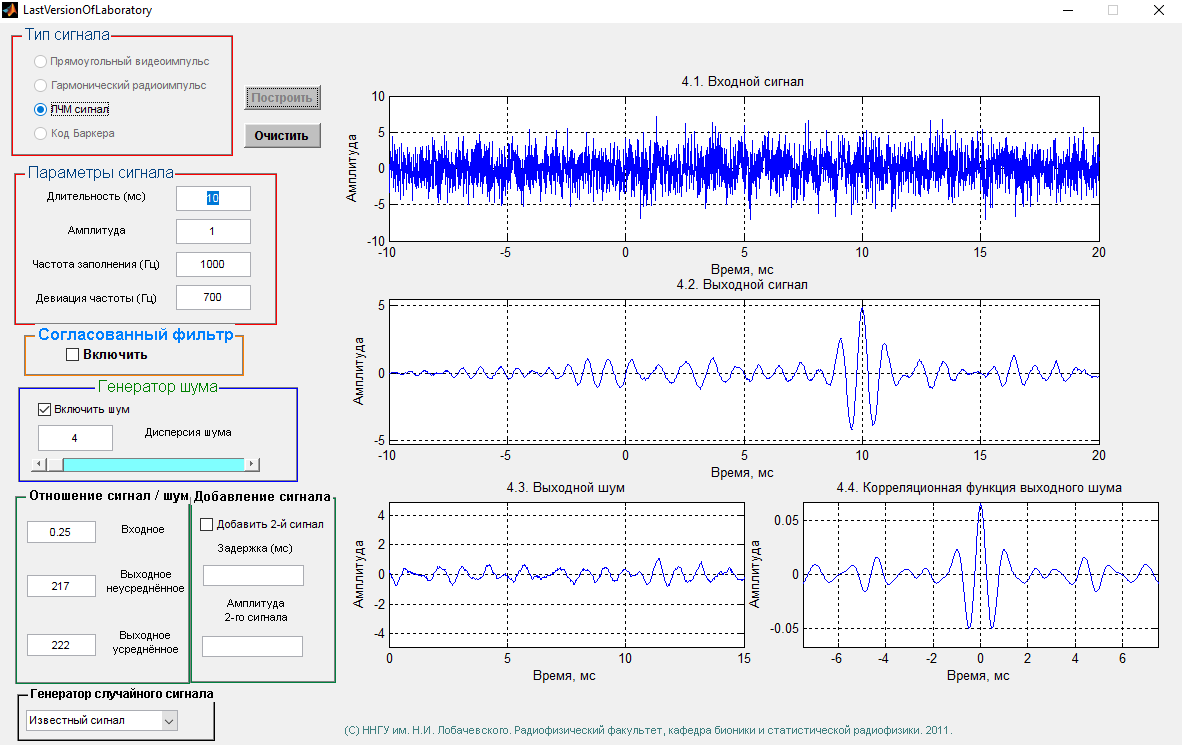
\includegraphics[width=\linewidth]{python/task4/t4s4_10_0}
    \caption{Панель виртуального прибора для задания 4.}
    \label{fig:4.1}
\end{figure}

Установили девиацию частоты $\Delta f_{\text{дев}}= 700$ Гц и изменяли
длительность в пределах 10 мс -- 100 мс. 


Был проведен эксперимент, в котором для нескольких реализаций виртуальным
прибором\footnote{Виртуальному прибору -- виртуальный студент}
вычислялось усредненное и неусредненное отношение сигнал/шум. Получившееся
облако точек представлено на рис.\ref{fig:4.1}.



\begin{figure}[h!]
    \centering
    %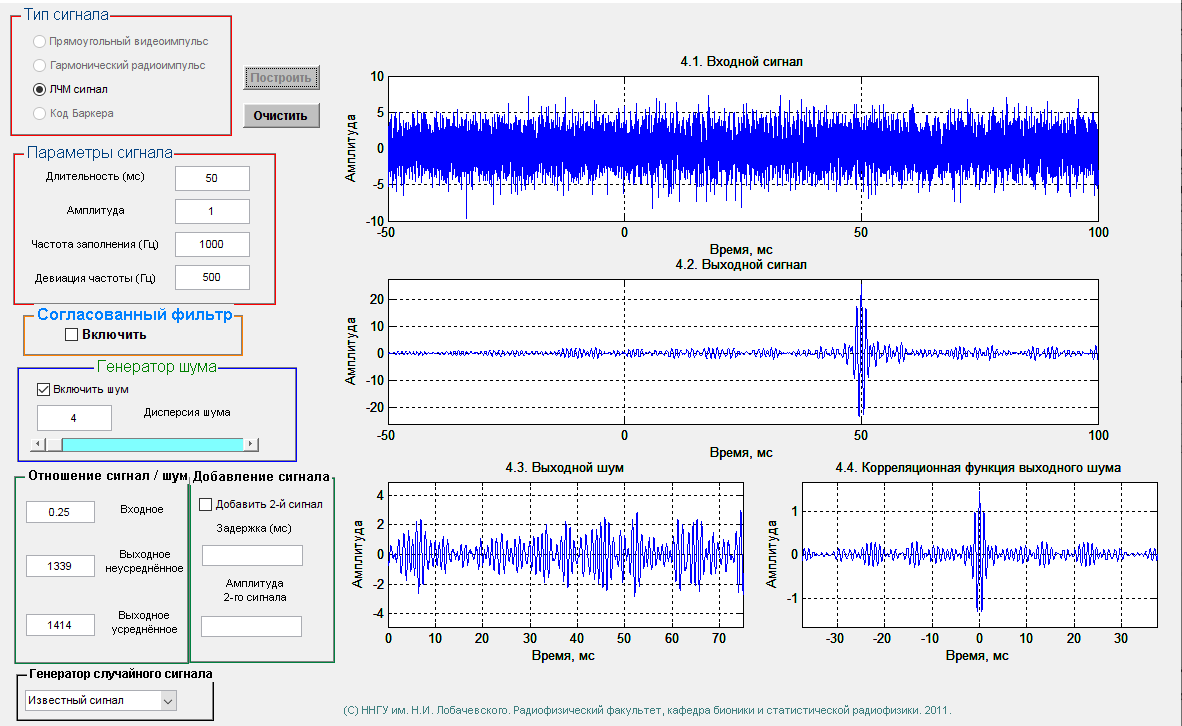
\includegraphics[width=0.6\linewidth]{imgs/t4s4_500}
    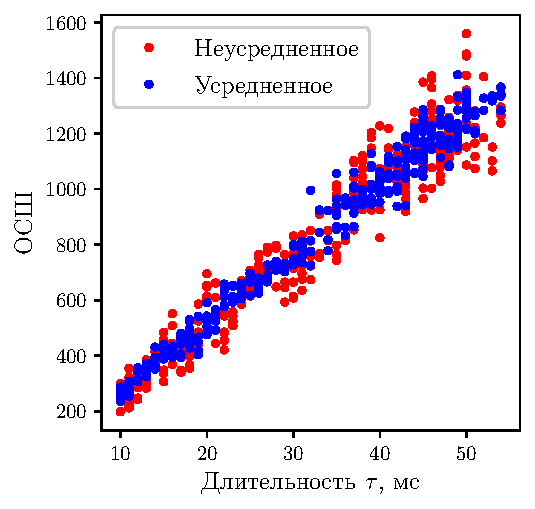
\includegraphics[width=0.6\linewidth]{imgs/task4/t4f1}
    \caption{Облако значений зависимости ОСШ от длительности $\tau$ ЛЧМ сигнала.} \label{fig:4.1}
\end{figure}


\newcommand{\mSNR}{\bar{\text{ОСШ}}}
Между реализациями, полученными при одинаковом значении длительности $\tau$
усреднялись, вычислялось среднее значение и формировалась усредненная функция
$\mSNR$ \footnote{Эт че, у меня двойное усреднение получается? Или
что такое в проге усредненное и неусредненное?}. Зависимость усредненного 
$\mSNR(\tau)$ от длительности сигнала представлена на рис. \ref{fig:4.2}.

\begin{figure}[h!]
    \centering
    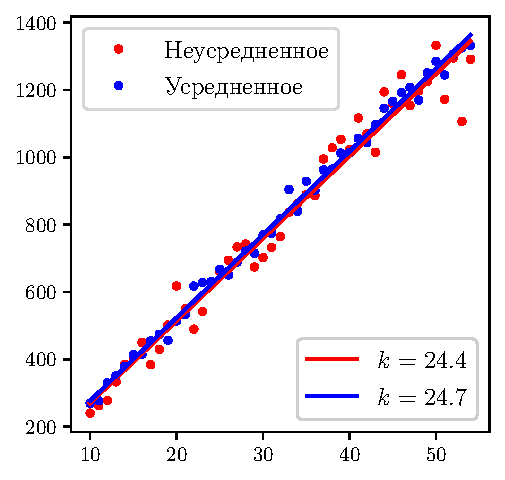
\includegraphics[width=0.6\linewidth]{imgs/task4/t4f2}
    \caption{Усредненная зависимость $\mSNR$ от длительности $\tau$ ЛЧМ сигнала. Сплошными линиями показана линейная
аппроксимация получившейся зависимости. Коэффициент $k$ обозначает коэффициент
наклона прямой}
    \label{fig:4.2}
\end{figure}

%\paragraph{Изменяющаяся девиация частоты ЛЧМ сигнала}%
%\label{par:izmeniaiushchaiasia_deviatsiia_chastoty_signala}
%Установили длительность сигнала $\tau=50$ мс и изменяли девиацию в пределах
%400 Гц - 1000 Гц.

%Для одной реализации сигнала виртуальным прибором
%вычислялось отношение сигнал/шум. Получившаяся зависимость приведена на рис.
%\ref{fig:4.2}









